\subsection{Summary of Completed Research}

We start with some definitions.
There are two basic ``quantity'' measures that
form the basis of our contribution measures:
$\txt(r)$ is the amount of text added in
revision $r$ of an article, and $\dist(r)$
is the edit distance of revision $r$ from
the revision previous to it.
There are also three basic ``quality'' measures
that we are able to define based on our previous
reputation research:
$\tlong(r)$ is a measure of the text longevity
of text added in revision $r$,
$\elong(r)$ is a measure of the edit longevity
of changes made for revision $r$,
and $\tenrevsq(r)$ simply is the sum of the amount
of text added in revision $r$ which is left over
in each of the ten revisions after $r$ divided by
the amount of text originally added.
We define $\editset(a)$ as the set of revisions
made by author $a$ across all pages.
This allows us to define the several contribution measures
presented in Table~\ref{tab-measures}.


\begin{table*}[!tp]
\begin{center}
\begin{tabular}{|rl|l|}
	\hline
\numedits(a) &$= \sum_{r\in\editset(a)} 1 \cdot 1 $&
	\text{Counts the number of edits made by the author.} \\
\textonly(a) &$= \sum_{r\in\editset(a)} 1 \cdot \txt(r)  $&
	\text{Counts the number of words added.} \\
\editonly(a) &$= \sum_{r\in\editset(a)} 1 \cdot \dist(r) $&
	\text{Sums the size of the edits made.} \\
\textlong(a) &$= \sum_{r\in\editset(a)} \tlong(r) \cdot \txt(r) $&
	\text{Sums the number of words added, factoring in quality.}\\
\editlong(a) &$= \sum_{r\in\editset(a)} \elong(r) \cdot \dist(r) $&
	\text{Sums the size of edits made, factoring in quality.}\\
\tenrevs(a)  &$= \sum_{r\in\editset(a)} \tenrevsq(r) \cdot \txt(r) $&
	\text{Sums the amount of text left over the next ten revisions.}\\
\hline
\end{tabular}
\end{center}
\caption[Contributions measures]{
This table presents the contribution measures we considered,
written so that each measure is clearly multiplying
``quality'' by ``quantity.''
}\label{tab-measures}
\end{table*}


\pagebreak
\subsection{Comparing Measures}

We next present the correlations between the various measures
in Table~\ref{cor-tab}.
These are correlations with respect to the amount of contributions
made by all non-anonymous authors, excluding those we've classified
as vandals.  
% \mynote{Vishwa: why did we exclude vandals?  Maybe we
% should explain.  -Bo}
%
\begin{sidewaystable}[!tp]
\begin{center}
\begin{tabular}{|c||c|c|c|c|c|c|c|}
	\hline
$Measures$ &  $EditLong$ & $EditOnly$ & $NumEdits$ & $TenRevs$ & $TextLong$ & $TextOnly$ & $TextWPen$ \\
        \hline \hline
$EditLong$         &  1.000  & 0.999  &  0.28  &         0.070  & 0.075  &  0.16  & -0.32 \\
$EditOnly$         &  0.999  & 1.000  &  0.29  &         0.071  & 0.077  &  0.16  & -0.33 \\
$NumEdits$         &  0.283  & 0.286  &  1.00  &         0.361  & 0.417  &  0.45  &  0.27 \\
$TenRevs$          &  0.070  & 0.071  &  0.36  &         1.000  & 0.983  &  0.96  &  0.89 \\
$TextLong$         &  0.075  & 0.077  &  0.42  &         0.983  & 1.000  &  0.98  &  0.90 \\
$TextOnly$         &  0.158  & 0.164  &  0.45  &         0.963  & 0.983  &  1.00  &  0.82 \\
$TextWPen$         & -0.320  &-0.326  &  0.27  &         0.886  & 0.897  &  0.82  &  1.00 \\
        \hline
\end{tabular}
\end{center}
\caption[Correlations of our measures]{
This table gives the pairwise correlations of the different measures we 
have defined in this paper.
}\label{cor-tab}
\end{sidewaystable}
%
From the correlation table, we notice that text based measures are
better positively correlated with each other.
Similarly, the edit based measures are better positively correlated 
with each other as we expected.
The measures $\editlong$ and $\editonly$ are highly correlated as 
borne out by the fact that a large percentage of the edits are of
good quality.
We notice that the same is true for $\textlong$ and $\textonly$.
The correlation between $\punish$ and the absolute measure
$\editonly$ is low, demonstrating that $\punish$
penalizes authors for bad edits, gives no credit to good edits,
and accumulates the quality discounted text contribution measure 
$\textlong$.
Therefore, authors need to contribute high quality text, while
ensuring that they have no bad edits to get a high score on
$\punish$.
$\tenrevs$ being a text contribution measure, is highly correlated
with the other text contribution measures $\textonly$ and
$\textlong$.
$\numedits$ is positively correlated with all measures as we would
expect, since the majority of contributions are deemed good by
each of the quality measures.

While $\textonly$ and $\editonly$ appear to be reasonable measures 
of author contribution, we have found evidence that vandals
accrue large contributions against these measures.
For instance, we found that author $1065172$ is in the $99th$ 
percentile when measured using $\textonly$, but is nearly at the
bottom of the ranks, at $0.000001$ quantile when we look at his
$\punish$ measure.
We found five revisions in which this author added new text, but
four of those were immediately reverted.
The only revision that was kept around was a one word addition to a
page!
From the edits made by this author, we saw that he is a spammer.
On the other hand, using $\textlong$ instead of $\textonly$ we
noticed that the author was below the $25th$ percentile.
On the $\editlong$ measure, this author was below the 
$0.001$ quantile; among the lowest in rank.
Therefore, we argue that the measures that discount $\textonly$ and 
$\editonly$ by a text or edit quality measure are more indicative
of the ``useful'' work added to the Wikipedia.
We argue that $\numedits$ is not as good a measure, since 
vandals and bots can easily make large numbers of bad edits.

We present two figures, Figure~\ref{fig-zoom-editonly-editlong}
and Figure~\ref{fig-zoom-textonly-textlong},
which have been restricted to a region containing the
bulk of the data points.
In Figure~\ref{fig-zoom-editonly-editlong},
we see a vee shape, which separates the authors into
two groups: those that have positive edit quality and those
that have negative edit quality, as measured by $\avgeditquality$.
The worse the quality of edits made by authors the less they
accumulate of the $\editlong$ measure, whereas the $\editonly$
measure, being oblivious to edit quality, attributes the same
contribution to an author whose contributions persists as it 
does to an author whose contributions do not.
On the negative side of $\editlong$, there are points that represent
vandals, who edit large sections of existing pages, which are
then immediately reverted.
Clearly, $\editonly$ ranks some of these authors very highly,
whereas $\editlong$ is able to distinguish them and rank
them very low.

In Figure~\ref{fig-zoom-textonly-textlong},
we see a similar vee shape; in this case, $\textlong$
cannot go below zero as the text quality measure is always 
non-negative, so vandals, by our definition, receive no 
contribution.
As before, the measure that incorporates quality can 
distinguish vandals from non-vandals and attribute a contribution
measure to authors that is proportional to the merit of their
contribution.

Of the various measures we introduced, $\punish$ is perhaps the
one with the least tolerance, since by this measure, the only way
an author can accumulate contribution is by adding new
text that persists and by making edits that are judged to be
of good quality.
Further, this measure does not reward authors for good edits,
but penalizes them for bad edits.
In Figure~\ref{fig-zoom-textonly-textwithpunish}, we plot $\textonly$
against $\punish$.
We see the vee shape, with vandals falling on a noticeable line in
the fourth quadrant, that has no $\textonly$ contribution.
Since almost all new text added by vandals is immediate reverted,
and their edits always have low quality, we notice that they get
low negative $\punish$ contributions.
In fact, we noticed that the bottom ten authors by rank when
measured according to $\punish$ were all vandals with the exception
of $AntiVandalBot$.
We explain this in the subsection on bots.

\begin{figure}[t]
    \begin{center}
    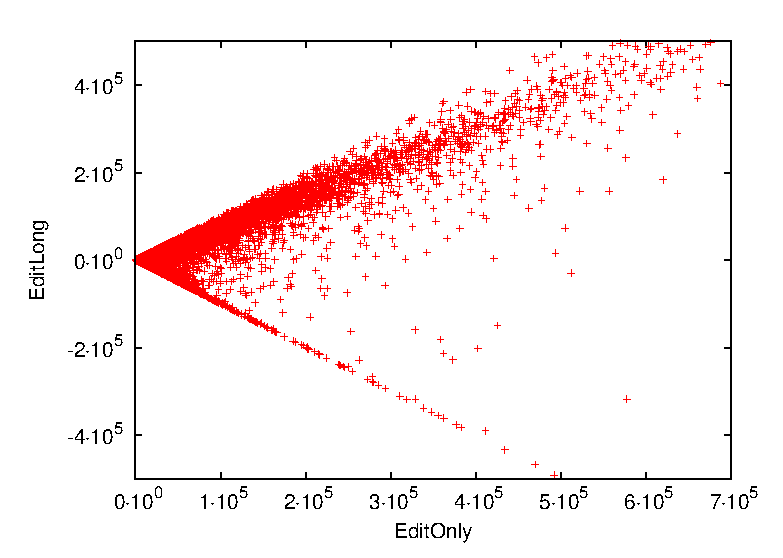
\includegraphics[width=0.70\textwidth]{part-I10-contrib/graphs/score-zoom-editonly-editlong}
    \end{center}
    \caption[EditOnly vs EditLong]{
    	Comparing the absolute edit contribution of a user
	with the edit longevity.
	Notice that authors who are ``all bad''
	are easily identifiable -- and sometimes quite prolific.
    }
    \label{fig-zoom-editonly-editlong}
\end{figure}
%
\begin{figure}[t]
    \begin{center}
    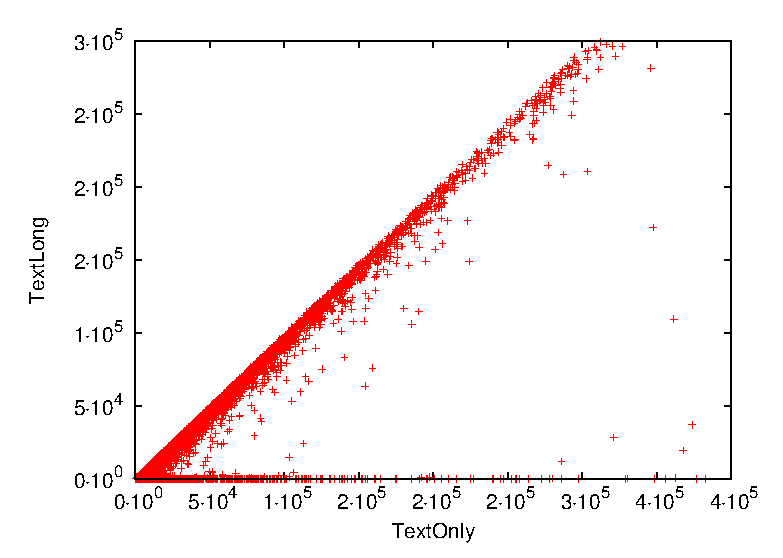
\includegraphics[width=0.70\textwidth]{part-I10-contrib/graphs/score-zoom-textonly-textlong}
    \end{center}
    \caption[TextOnly vs TextLong]{
    	Comparing the absolute text contribution with the contribution
	as measured by text longevity.
	We see that large contributors are either ``all bad''
	or nearly ``all good.''
    }
    \label{fig-zoom-textonly-textlong}
\end{figure}
%
\begin{figure}[t]
    \begin{center}
    \includegraphics[width=0.70\textwidth]{part-I10-contrib/graphs/score-zoom-textonly-textwithpunish}
    \end{center}
    \caption[TextOnly vs TextWithPunish]{
    	Comparing the absolute text contribution of an author with
	their contribution as measured by \punish.
    }
    \label{fig-zoom-textonly-textwithpunish}
\end{figure}
%
\begin{figure}[t]
    \begin{center}
    \includegraphics[width=0.70\textwidth]{part-I10-contrib/graphs/score-zoom-revisions-textonly}
    \end{center}
    \caption[Measuring short term text survival]{
    	This graph compares how much text is initially added
	by a user (along the $x$-axis), with how much
	of the text survives over the next ten filtered revisions
	(along the $y$-axis).
	The higher up the $y$-axis a point is, the more
	text that survived all ten revisions.
	Most authors add under 100,000 words,
	and about half of what they add survives.
    }
    \label{fig-zoom-revisions-textonly}
\end{figure}

\subsection{Ranking Authors}

A different direction we explored was how these different
measures end up ranking different authors.
Since the contribution measures varied over such a
wide range of values, with most people within
a smaller region around zero, we hoped that
ranking the authors would give us better insight into how
the measures differed.

To this end,  we computed the percentile rank
(rounded up to the next even value for clarity in the image)
of all non-anonymous authors, including those
that we had classified as vandals, and then plotted
them in 3-dimensional histograms; see
Figures~\ref{fig-prct-editlong-textlong}
and~\ref{fig-prct-editlong-textwithpunish}.
An important point to remember about
Figures~\ref{fig-prct-editlong-textlong}
and~\ref{fig-prct-editlong-textwithpunish}
is that the low-lying regions of the graph are
rarely zero --- there are roughly between one and ten
authors at each intersection, but this is so small compared
to the areas that correlate that we cannot see it on the graph.
Both figures show a high degree of correlation that wasn't evident
from the correlation scores in Table~\ref{tab:measure-correlations}.
Figure~\ref{fig-prct-editlong-textlong} shows that \textlong and
\editlong generally agree in the ranking of users, except for the lowest
scorers of \textlong.
The lowest scorers of \textlong all receive a score of zero, but the
``fence'' seen in the figure is an indication of the fact that there are
an enormous number of users which \textlong ranks equivalently but
\editlong is able to further distinguish between.
By contract, Figure~\ref{fig-prct-editlong-textwithpunish} shows that
\punish roughly agrees with \editlong for all users except for a thin
branch that score zero under \punish but get a positive score under
\editlong.
This thin branch represents the group of users which do not add text,
but instead only rearrange it or delete vandalism.
%
\begin{figure}[tbhp]
    \begin{center}
    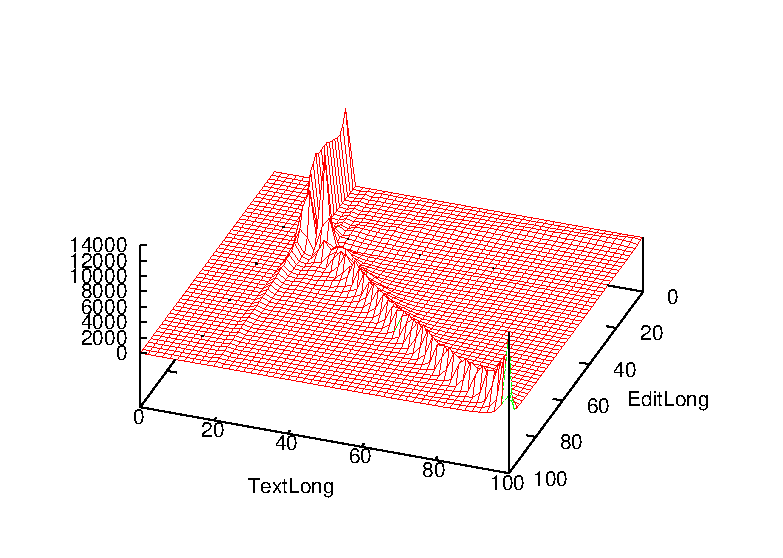
\includegraphics[width=0.85\textwidth]{part-I10-contrib/graphs/prct-editlong-textlong}
    \end{center}
    \caption[Comparing edit longevity with text longevity]{
    	$\editlong$ vs $\textlong$
    }
    \label{fig-prct-editlong-textlong}
\end{figure}
%
\begin{figure}[tbhp]
    \begin{center}
    \includegraphics[width=0.85\textwidth]{part-I10-contrib/graphs/prct-editlong-textwithpunish}
    \end{center}
    \caption[Comparing edit longevity with the punishing function]{
    	$\editlong$ vs $\punish$
    }
    \label{fig-prct-editlong-textwithpunish}
\end{figure}
%

We also include a 3-dimensional histogram comparing the
percentile rankings as determined by \editlong and \numedits,
in Figure~\ref{fig-prct-editlong-numedits}.
The ``rows of fences'' we see
in Figure~\ref{fig-prct-editlong-numedits}
are due to the large number of authors who
make only a handful of edits; the \numedits measure
neither distinguishes them from each other,
nor is it capable of distinguishing good contributions from
bad contributions.
This last point is important, that even users in
the lowest percentile of \editlong can be rated
very highly by \numedits --- demonstrating
that it is much easier to game the \numedits
measure to achieve a high rank, while doing bad work.
%
\begin{comment}
%
\begin{figure}[tbhp]
    \begin{center}
    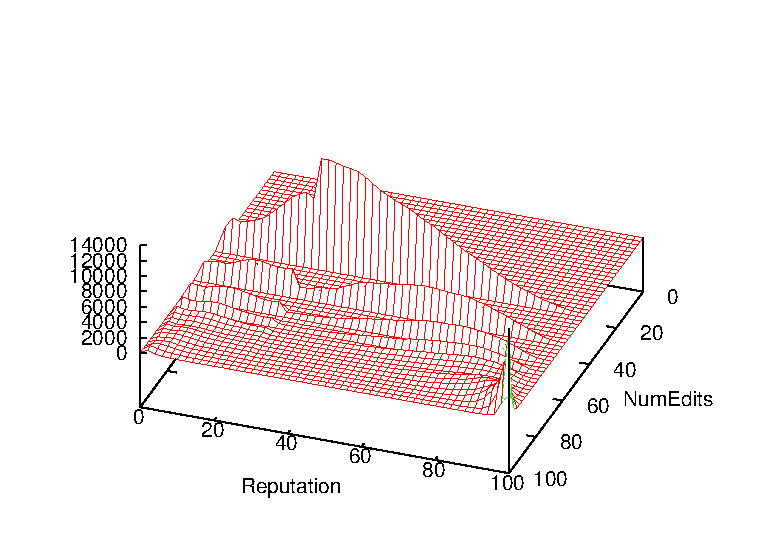
\includegraphics[width=0.85\textwidth]{part-I10-contrib/graphs/prct-numedits-reputation}
    \end{center}
    \caption[Comparing the number of edits made with the reputation function]{
    	The \contribrep measure had the highest correlation to \numedits,
	in Table~\ref{tab:measure-correlations}.
	Notice that \numedits does not distinguish well
	between users.
    }
    \label{fig-prct-numedits-reputation}
\end{figure}

\begin{figure}[tbph]
    \begin{center}
    \includegraphics[width=0.85\textwidth]{part-I10-contrib/graphs/prct-editlong-reputation}
    \end{center}
    \caption[Comparing edit longevity with reputation]{
    	\editlong vs \contribrep
    }
    \label{fig-prct-editlong-reputation}
\end{figure}
%
\end{comment}

\begin{figure}[tbph]
    \begin{center}
    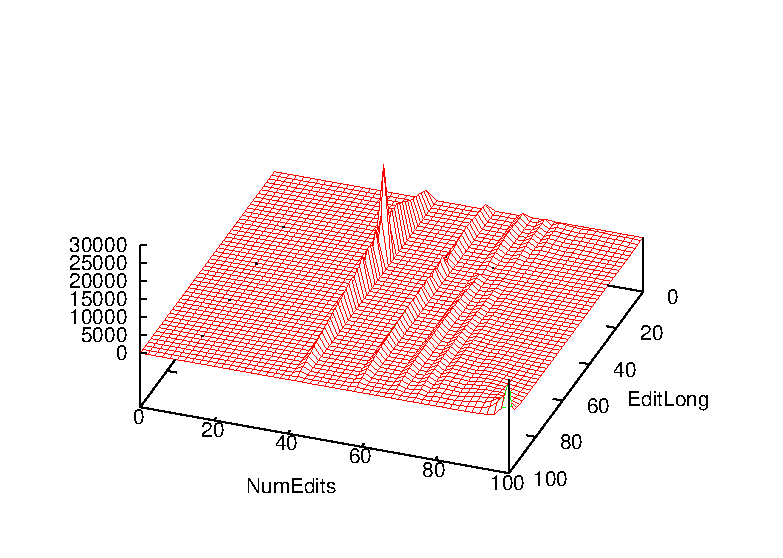
\includegraphics[width=0.85\textwidth]{part-I10-contrib/graphs/prct-editlong-numedits}
    \end{center}
    \caption[Comparing edit longevity with the number of edits made]{
    	$\editlong$ vs $\numedits$
    }
    \label{fig-prct-editlong-numedits}
\end{figure}


